Nearly all data sets of interest for analytics can be modeled as data cubes. There is immense potential value in data that is not being realized because it is difficult to combine data sets together from multiple sources and visualize the integrated structure. Our proposed data representation framework, called the Universal Data Cube (UDC), provides solutions for:
\begin{itemize}
\item modeling existing data sets as data cubes,
\item integrating the data sets together, and
\item querying the integrated data structure for interactive visualization.
\end{itemize}
\section{Terminology and Data Structures}
A data cube is a multidimensional data structure that organizes data into \emph{dimensions} and \emph{measures}. Dimensions are sets of distinct entities that may be unordered, ordered, or hierarchical. Each distinct entity of a dimension is called a \emph{member}. Measures are aggregated quantitative values that can be assigned to combinations of dimension members called \emph{cells}. An \emph{observation} links a cell with concrete values for one or more measures. A \emph{data cube}, also referred to as simply a \emph{cube}, is a set of observations that draw from a common set of dimensions and measures. The table below provides examples for each of the terms introduced.

\begin{center}
  \begin{tabular}{ | c | c | }
    \hline
    \textbf{Term} & \textbf{Examples} \\ \hline
    dimension & Space, Time \\ \hline
    member & India, China, 1970, 2010 \\ \hline
    measure & Population, Gross Domestic Product\\ \hline
    cell & India in 1970, China in 2010 \\ \hline
    observation & The population of India in 1970 was 555.2 million. \\ \hline
    cube & The population of India in 1970 was 555.2 million. \\
         & The population of India in 2010 was 1,206 million. \\
         & The population of China in 1970 was 818.3 million. \\
         & The population of China in 2010 was 1338 million. \\ \hline
  \end{tabular}
\end{center}

Existing data cube technologies do not readily support integration of data cubes from multiple sources. Many data sets can be modeled as data cubes that have dimensions and measures in common. The dimensions and measures they have in common can be utilized to integrate multiple data cubes together into a unified structure. The difficulty in integrating data cubes from multiple sources arises from different identifiers referring to the same member and different scale factors being used for the same measure. Our data cube representation and integration framework, called the \emph{Universal Data Cube} (UDC), addresses these difficulties.

In order to account for different identifiers referring to the same member, we introduce the concept of a \emph{code list}. A code list is a family of identifiers, also called \emph{codes}, that refer to members \cite{rdfdatacube}. A \emph{concordance table}, also referred to as simple a \emph{concordance}, is a table that declares equivalences between codes from different code lists \cite{doan2012principles}. Members can be identified unambiguously as (dimension, code list, code) tuples called \emph{qualified members}. The table below provides examples for each of the terms introduced. 
\begin{center}
  \begin{tabular}{ | c | c | }
    \hline
    \textbf{Term} & \textbf{Example} \\ \hline
    code list & Country Name, Country Code \\ \hline
    code & India, in \\ \hline
    qualified member & (Space, Country Code, in) \\
                     & (Space, Country Name, China) \\ \hline
    concordance table &
      \begin{tabular}{ c c }
        \textbf{Country Name} & \textbf{Country Code} \\
        India & in \\
        China & cn
      \end{tabular} \\ \hline
  \end{tabular}
\end{center}

Data tables can contain data that can be modeled as either a cube or a concordance. In either case, columns in the tables can be either \emph{dimension columns} or \emph{measure columns}. A dimension column contains codes from a single code list. A measure column contains numbers representing values for a certain measure. Values in a measure column may be scaled (multiplied by a scaling factor). In order to be imported into the UDC framework, data tables must be annotated with metadata that declares whether the table represents a cube or a concordance, and specifies the role of each column as either a dimension column or a measure column. Below are some concrete examples of data tables and their metadata.

\begin{center}
  \begin{tabular}{ | c | c | c | }
    \hline
    \textbf{countryCode} & \textbf{year} & \textbf{gdp} \\ \hline
    IND & 1960 & 37679274491.2745 \\ \hline
    IND & 2010 & 1708450861364.17 \\ \hline
    CHN & 1960 & 61377930682.0013 \\ \hline
    CHN & 2010 & 5930529470799.17 \\ \hline
    USA & 1960 & 520531181568 \\ \hline
    USA & 2010 & 14958300000000 \\ \hline
  \end{tabular}
\end{center}

\begin{codebox}
\li   $dimensionColumns: [$
\Do
\li     $\{column:$\verb1'countryCode'1$, dimension:$\verb1'Space'1$, codeList:$\verb|'ISO3'|$\},$
\li     $\{column:$\verb1'year'1$, dimension:$\verb1'Time'1$, codeList:$\verb|'Year'|$\}$
\End
\li   $ ]$
\li   $measureColumns: [$
\Do
\li     $\{column:$\verb1'gdp'1$, measure:$\verb1'Gross Domestic Product'1$\}$
\End
\li   $ ]$
\end{codebox}

\begin{center}
  \begin{tabular}{ | c | c | c | }
    \hline
    \textbf{countryName} & \textbf{unCountryCode}& \textbf{alphaCode} \\ \hline
    India & 356 & IND \\ \hline
    China & 156 & CHN \\ \hline
    United States of America & 840 & USA \\ \hline
  \end{tabular}
\end{center}

\begin{codebox}
\li   $dimensionColumns: [$
\Do
\li     $\{column:$\verb1'countryName'1$, dimension:$\verb1'Space'1$, codeList:$\verb|'UN Geoname'|$\},$
\li     $\{column:$\verb1'unCountryCode'1$, dimension:$\verb1'Space'1$, codeList:$\verb|'UN M.49'|$\},$
\li     $\{column:$\verb1'alphaCode'1$, dimension:$\verb1'Space'1$, codeList:$\verb|'ISO3'|$\}$
\End
\li   $ ]$
\end{codebox}

\begin{center}
  \begin{tabular}{ | c | c | c | }
    \hline
    \textbf{countryCode} & \textbf{year}& \textbf{pop} \\ \hline
    356 & 1960 & 449595.489 \\ \hline
    356 & 2010 & 1205624.648 \\ \hline
    156 & 1960 & 650680.114 \\ \hline
    156 & 2010 & 1359821.465 \\ \hline
    840 & 1960 & 186361.893 \\ \hline
    840 & 2010 & 312247.116 \\ \hline
  \end{tabular}
\end{center}

\begin{codebox}
\li   $dimensionColumns: [$
\Do
\li     $\{column:$\verb1'countryCode'1$, dimension:$\verb1'Space'1$, codeList:$\verb|'UN M.49'|$\},$
\li     $\{column:$\verb1'year'1$, dimension:$\verb1'Time'1$, codeList:$\verb|'Year'|$\}$
\End
\li   $ ]$
\li   $measureColumns: [$
\Do
\li     $\{column:$\verb1'pop'1$, measure:$\verb1'Population'1$\}$
\End
\li   $ ]$
\end{codebox}

\TODO{ Explain the above examples. }
\TODO{ Add the following sections: }

Loading Concordances

Member Canonicalization 

Loading Cubes

Cube Canonicalization 

Merging Cubes

Querying Cubes

Cube Projection

Hierarchies

Drill Down and Roll Up

\section{Data Sets}
\subsection{United Nations Population Estimates}
\subsection{World Bank World Development Indicators}
\begin{figure}[h]
  \caption{The World Bank Web page for their data table containing Gross Domestic Product for world countries.}
  \centering
  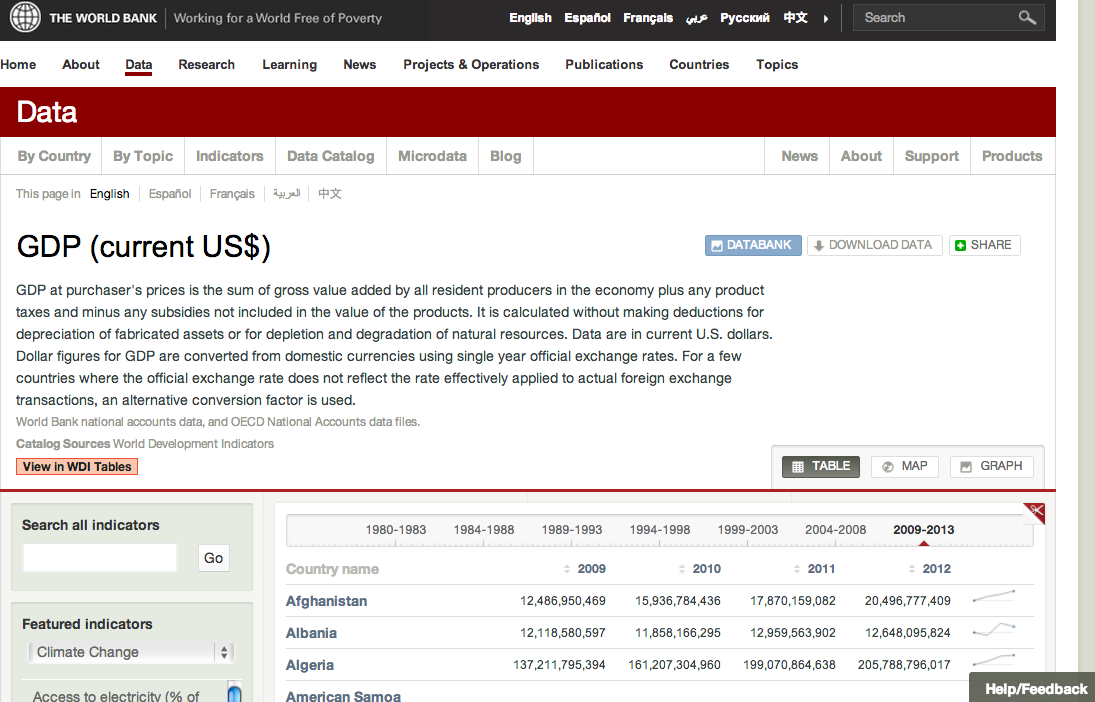
\includegraphics[width=\textwidth]{figures/worldBankGDP.png}
\end{figure}
\subsection{United Nations Millenium Development Goals}
\subsection{United States Census Population Estimates}
\begin{figure}[h]
  \caption{A screenshot of the US Census Population by State data set. This data set is made available in Excel and CSV formats.}
  \centering
  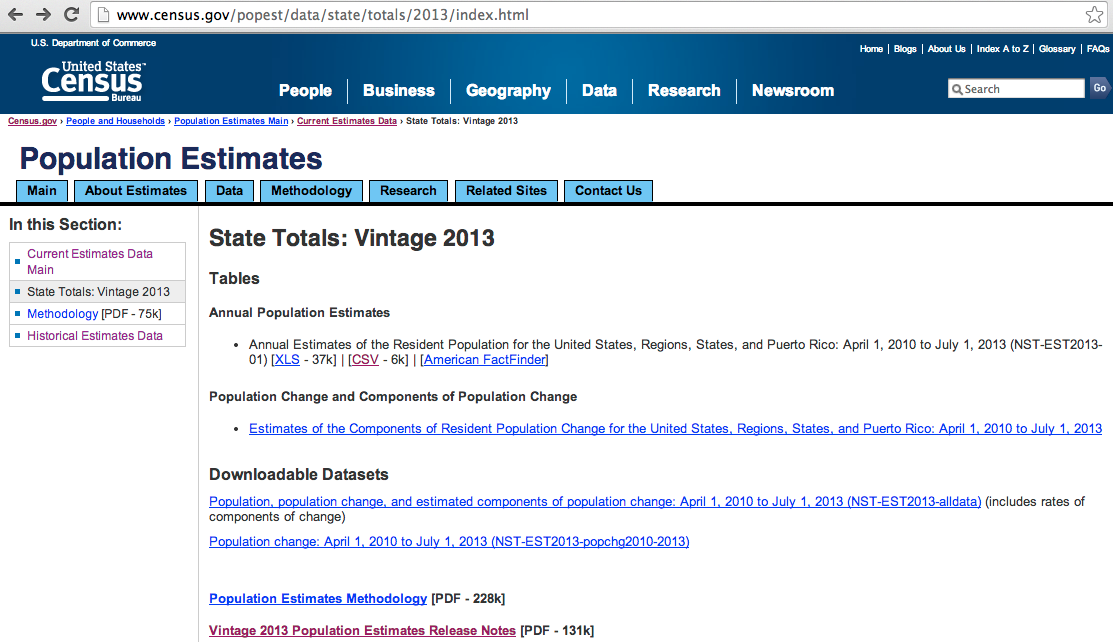
\includegraphics[width=\textwidth]{figures/usCensusPopulationByState.png}
\end{figure}
\TODO{ import data from http://www.census.gov/popest/data/state/totals/2013/index.html}

\subsection{US Central Intelligence Agency World Factbook}
\TODO{ import subsets of the data}
\subsection{US Centers for Disease Control Causes of Death}
\TODO{ generalize stacked area and tree vis}
\subsection{W3Schools Browser Market Share}
\TODO{ import this data completely}
\subsection{Natural Earth}
\begin{figure}[h]
  \caption{A screenshot of the Natural Earth geographic data Web site.}
  \centering
  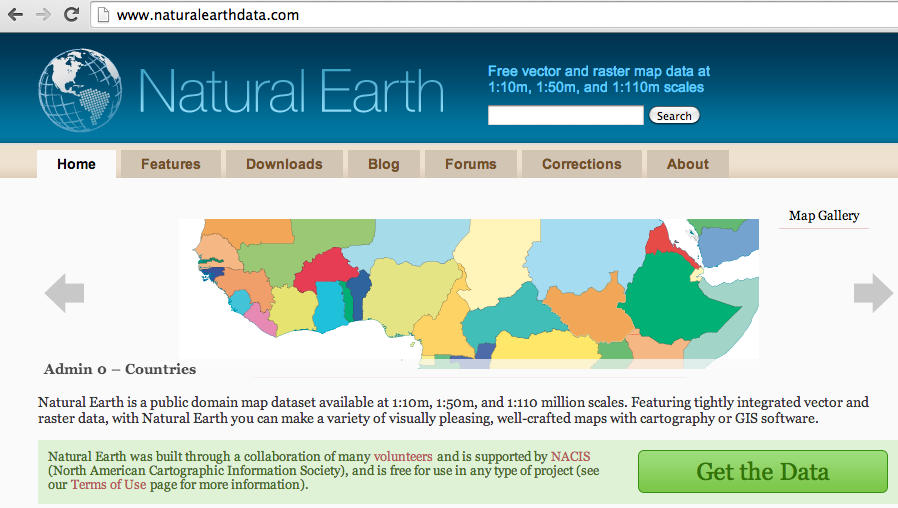
\includegraphics[width=\textwidth]{figures/naturalEarth.png}
\end{figure}
\TODO{ discuss data transformation process }
